%! Author = Yannis Teissier \& Wolodia Zdetovetzky
%! Date = 04/2023
\documentclass{article}

\usepackage[utf8]{inputenc}
\usepackage[T1]{fontenc}
\usepackage{amsmath}
\usepackage{listings}
\usepackage{graphicx}
\usepackage{hyperref}
\inputencoding{utf8}

\title{Massive data processing \\ with the Unsplash dataset}
\author{Yannis TEISSIER \& Wolodia ZDETOVETZKY}
\date{03/2023}


\begin{document}

    \maketitle
    \tableofcontents
    \newpage


    \section{Objectives}\label{sec:objectives}

    In this project, we aimed to develop a comprehensive image recommendation system based on the Unsplash image dataset, taking into account user preferences.
    The following steps explain the objectives we pursued in order to achieve this goal.

    \textbf{Data Collection}\\
    Our first objective was to efficiently collect and process the large volume of data available in the Unsplash image dataset.
    We achieved this by parallelling the download process across multiple processes to enhance performance.

    \textbf{Data Annotation}\\
    To enrich the dataset, we aimed to automatically annotate the images with relevant metadata.
    This involved using Facebook's Detr AI for image recognition, which allowed us to generate descriptive tags for each image.

    \textbf{Dominant Color Extraction}\\
    We aimed to identify the four most dominant colors in each image to further enrich the metadata.
    To achieve this, we employed the K-means clustering algorithm,
    which allowed us to determine the most representative colors in each image effectively.

    \textbf{Data Visualization}\\
    We sought to expand the data visualization capabilities to align with the most relevant metadata obtained during the annotation and color extraction processes.
    This objective aimed to facilitate a better understanding of the dataset characteristics and user preferences.

    \textbf{Recommendation System Development}\\
    A central objective of this project was the development of an effective image recommendation system.
    We explored various techniques, such as Euclidean distance, cosine similarity, and Reinforcement Learning, to identify the best approach for providing personalized image recommendations to users.

    \textbf{Web Interface Implementation}\\
    The creation of a user-friendly web interface was our objective, enabling users to define their profiles and receive image recommendations.

    In annexe, you will find the~\hyperref[subsec:target_architecture]{\nameref{subsec:target_architecture}} proposed by the initial subject, followed by the~\hyperref[subsec:actual_architecture]{\nameref{subsec:actual_architecture}} of the project.

    \newpage


    \section{Data}\label{sec:data}

    \subsection{Data Source}\label{subsec:data_source}
    For our data source, we decided to use the Unsplash dataset (\url{https://github.com/unsplash/datasets}).
    This dataset consists of over 250,000 images contributed by photographers with diverse contexts, subjects, and use cases.

    \subsection{Licensing}\label{subsec:licensing}
    As stated on their website, Unsplash grants a worldwide, irrevocable, and non-exclusive copyright license for
    downloading, copying, modifying, distributing, reproducing, displaying, and using Unsplash photos free of charge, including for commercial purposes, without requiring additional permission from the photographer or Unsplash.
    This license does not include the right to compile Unsplash photos to replicate a similar or competing service.
    It is also worth mentioning that attributing credit is appreciated to help grow their community.
    Regarding the datasets, the Lite version is available for both commercial and non-commercial use.
    However, the complete dataset is intended for non-commercial use only.

    \subsection{Data Size}\label{subsec:data_size}
    In terms of data dimensions, Unsplash offers more than 3 million curated images, thanks to a community of nearly 300,000 professional and amateur photographers.
    The Lite dataset contains 25k nature-themed photos, 25k keywords, and 1 million searches.
    The complete dataset contains over 3 million high-quality photos, 5 million keywords, and more than 250 million searches.

    \subsection{Stored Information}\label{subsec:stored_infos}
    We store all the extracted metadata for the images in our database, along with the generated tags and dominant colors for each image.
    The following is a list of the stored fields: filename, Make, Model, Software, BitsPerSample, ImageWidth, ImageHeight, ImageDescription, Orientation, Copyright, DateTime, DateTimeOriginal, DateTimeDigitized, SubSecTimeOriginal, ExposureTime, FNumber, ExposureProgram, ISOSpeedRatings, SubjectDistance, ExposureBiasValue, Flash, FlashReturnedLight, FlashMode, MeteringMode, FocalLength, FocalLengthIn35mm, Latitude, LatitudeDegrees, LatitudeMinutes, LatitudeSeconds, LatitudeDirection, Longitude, LongitudeDegrees, LongitudeMinutes, LongitudeSeconds, LongitudeDirection, Altitude, DOP, FocalLengthMin, FocalLengthMax, FStopMin, FStopMax, LensMake, LensModel, FocalPlaneXResolution, FocalPlaneYResolution, tags, dominant\_color.
    In addition to the metadata, we store the images themselves in a Minio database.
    Minio is a high-performance, secure, and scalable object storage solution.

    \subsection{User preferences}\label{subsec:user_pref}
    Through the web interface, we collect user data to provide personalized image recommendations.
    Users are asked to fill in various fields, such as their favorite color using a color picker (which yields a hexadecimal code),
    desired image dimensions (height and width), orientation (landscape or portrait),
    tags representing the elements they wish to visualize (up to a maximum of 5), and the preferred camera make.
    This information is then used to generate recommendations that align with the user's preferences.


    \section{Data exploration}\label{sec:exploration}

    \subsection{Used models}\label{subsec:models}



    \subsection{Obtained metrics}\label{subsec:metrics}


    \section{Auto-evaluation}\label{sec:autoeval}


    \section{Remarques}\label{sec:remarques}

    \subsection{Séances pratiques}\label{subsec:seances}

    \subsection{Exercices}\label{subsec:exercices}

    \subsection{Améliorations}\label{subsec:ameliorations}


    \section{Conclusion}\label{sec:conclusion}

    \newpage
    \appendix


    \section{Annexe}\label{sec:annexe}

    \subsection{target architecture}\label{subsec:target_architecture}

    \begin{figure}[htbp]
        \centering
        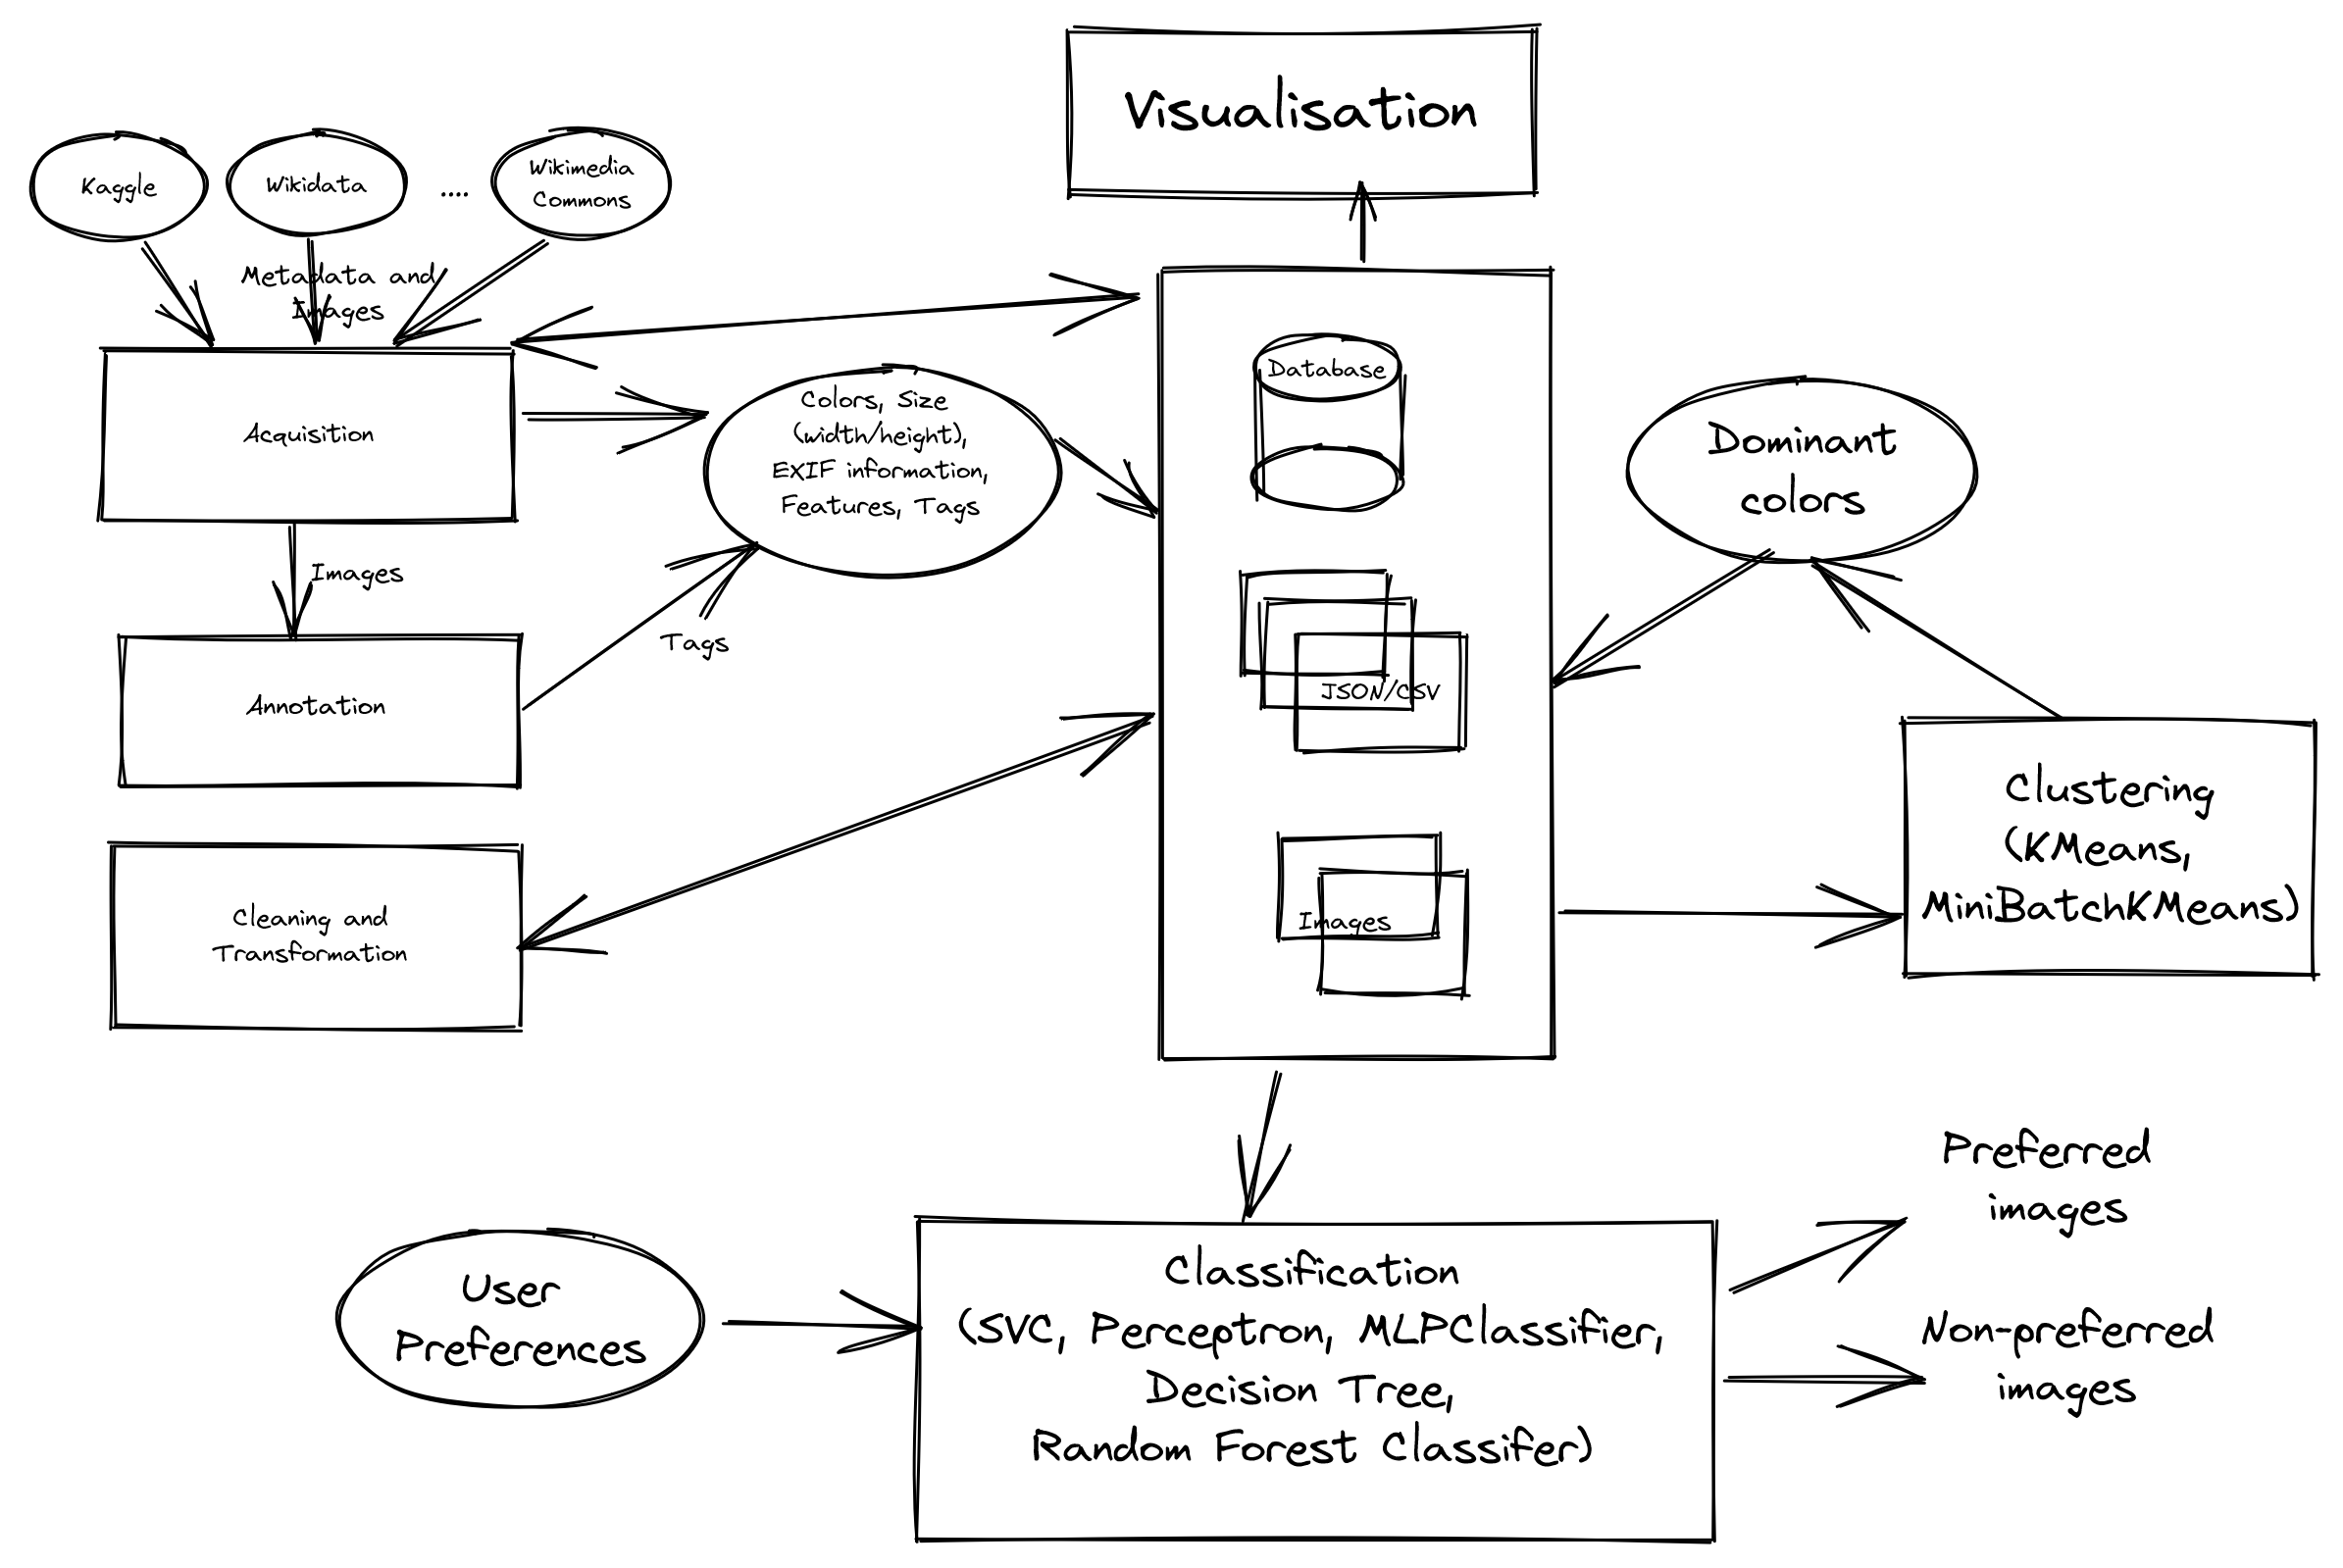
\includegraphics[width=0.7\textwidth]{targeted_archi}
        \caption{Targeted architecture}
        \label{fig:targeted_architecture}
    \end{figure}

    \subsection{actual architecture}\label{subsec:actual_architecture}

    \begin{figure}[htbp]
        \centering
        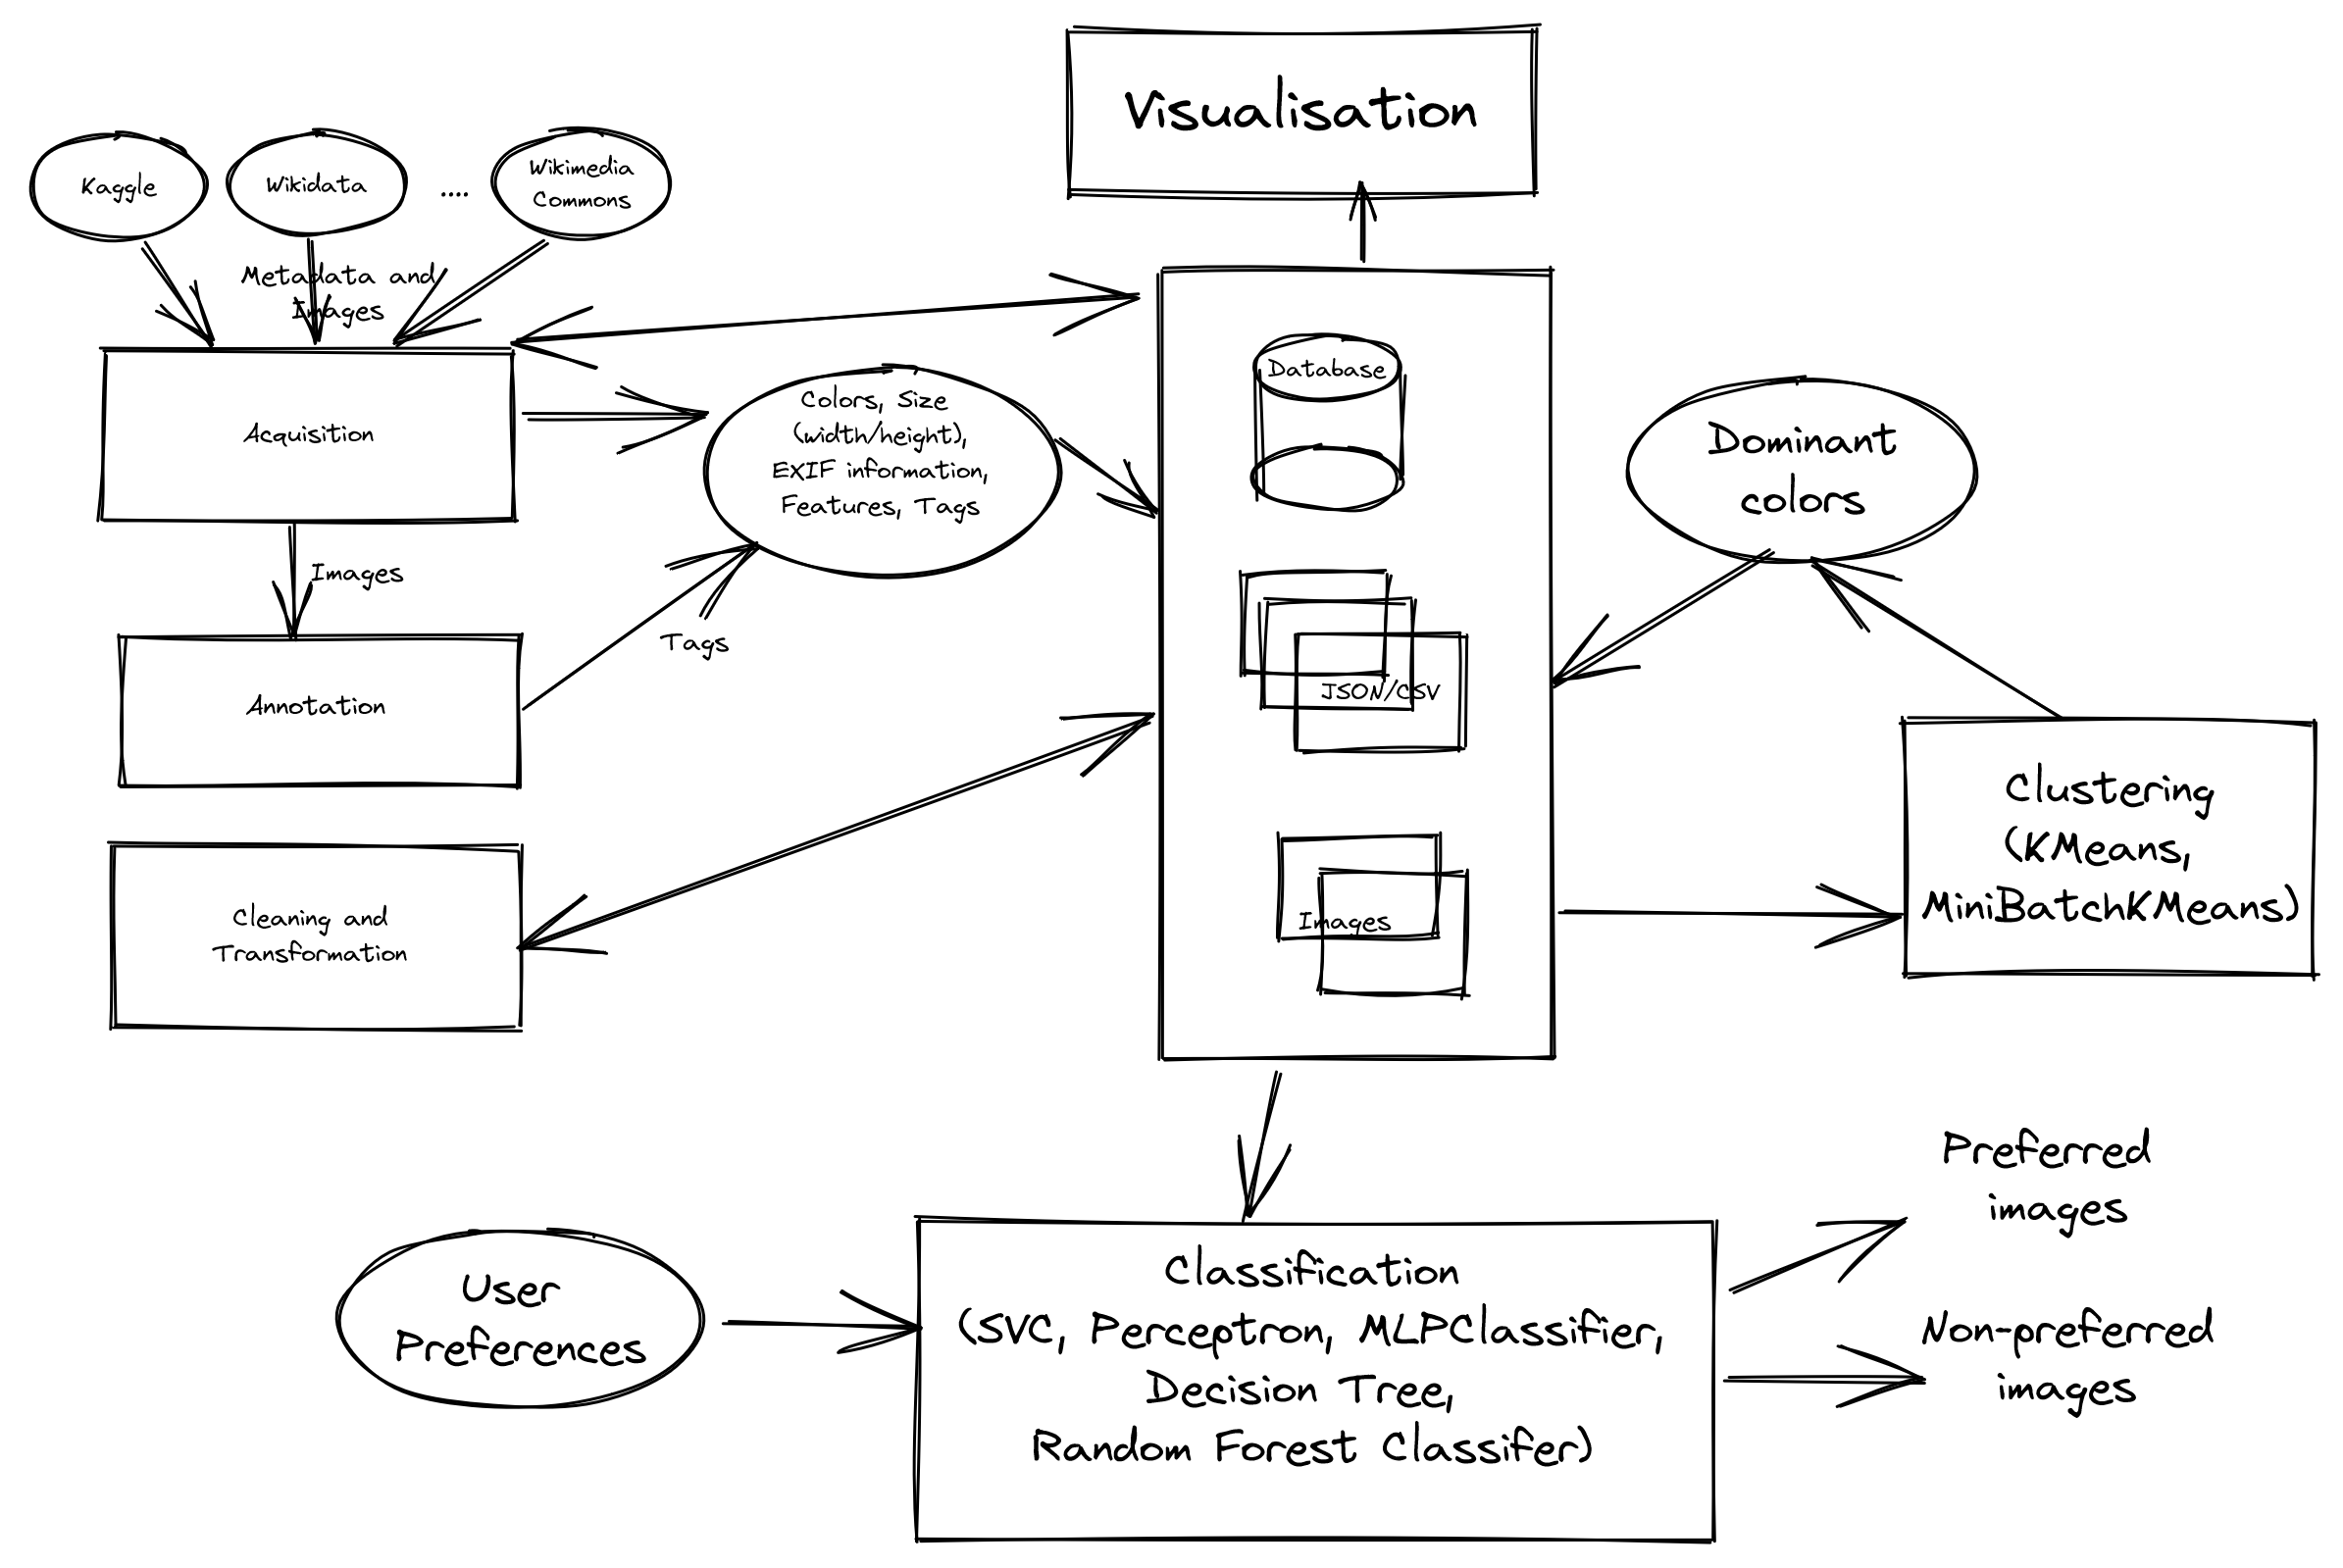
\includegraphics[width=0.7\textwidth]{targeted_archi} % TODO : create the actual one
        \caption{Actual architecture}
        \label{fig:actual_architecture}
    \end{figure}


\end{document}



